
\subsection*{task 3.3 [10 points] \\[1ex] fastmap}

In the \texttt{Data} folder for this exercise, you will find the file
\begin{quote}
    \texttt{faceMatrix.npy}
\end{quote}
which contains a data matrix $\mat{X} \in \mathbb{R}^{361 \times 2429}$ whose columns $\vec{x}_i$ represent tiny face images of size $19 \times 19$ pixels. To read this matrix into memory and check its size, you may use
\begin{python}
matX = np.load('faceMatrix.npy').astype('float')
m, n = matX.shape
print (m, n)
\end{python}
To have a look at one of the images it contains, say $\vec{x}_{15}$, you may use this
\begin{python}
vecX = matX[:,14].reshape(19,19)
plt.imshow(vecX, cmap='gray')
plt.xticks([])
plt.yticks([])
plt.show()
\end{python}
\vspace{2cm}


Having read matrix $\mat{X}$ into memory, here is what you are supposed to do:

\begin{enumerate}
\item Implement the \emph{fastmap} algorithm which we discussed in lecture 07. Recall that this algorithm involves a function \textsc{getDistantObjects}. How would you implement it in numpy / scipy?
%%%%%
%%%%%
%%%%% enter your code into the following environment
%%%%%
%%%%%
\begin{python}
# helper function to compute the squared norm of vectors
sq_norm = lambda X: (X ** 2).sum(axis=0)
# function implementing fastmap
def fastmap(
    X:np.ndarray, 
    k:int
) -> np.ndarray:
    m, n = X.shape
    # list of the computed approximations
    V = []
    # do the iterations
    for _ in range(k):
        # find the two most distant object indices
        i = np.random.choice(n, size=1)[0]
        j = sq_norm(X - X[:, i:i+1]).argmax()
        i = sq_norm(X - X[:, j:j+1]).argmax()
        j = sq_norm(X - X[:, i:i+1]).argmax()
        # approximate the major component of the current matrix X
        v = (X[:, j:j+1] - X[:, i:i+1])
        v /= la.norm(v, axis=0)
        # add the major component to the list
        V.append(v)
        # project vectors into subspace
        X = (np.eye(m) - v @ v.T) @ X
    # stack all approximations and return
    return np.concatenate(V, axis=1)
\end{python}
%%%%%
%%%%%
%%%%%
%%%%%
%%%%%

\item Run your \emph{fastmap} implementation to obtain approximations of the top $25$ principal components of the data in matrix $\mat{X}$. 
\begin{python}
# compute approximations of major components using fastmap
V = fastmap(X, k=25)
\end{python}

\item  Compute the SVD of matrix $\mat{X}$ and determine the top $25$ left singular vectors.
\begin{python}
# compute the left singular vectors of the data matrix using svd
U, _, _ = la.svd(X)
# get only the first 25 singular vectors and ignore the rest
# note that the singular values are sorted in non-increasing order
# thus the first k singular vectors are the first k major components
U = U[:, :25]
\end{python}

\item Compare your \emph{fastmap} results to your SVD results. A good idea for doing this is to visualize / plot them as tiny images; figure out how to create a plot that shows not just a single tiny image but $25$ at the same time

%%%%%
%%%%%
%%%%% enter plots here, i.e. replace "placeholder.pdf" by the name of the graphics files you created
%%%%%
%%%%%
\begin{center}
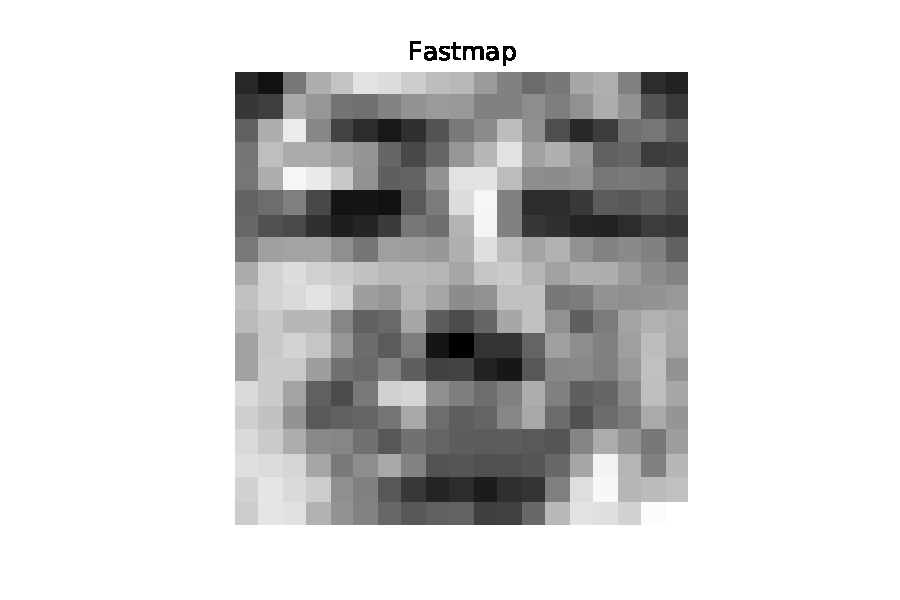
\includegraphics[width=0.45\textwidth]{Ex_03/Figures/fastmap.pdf}
\hfill
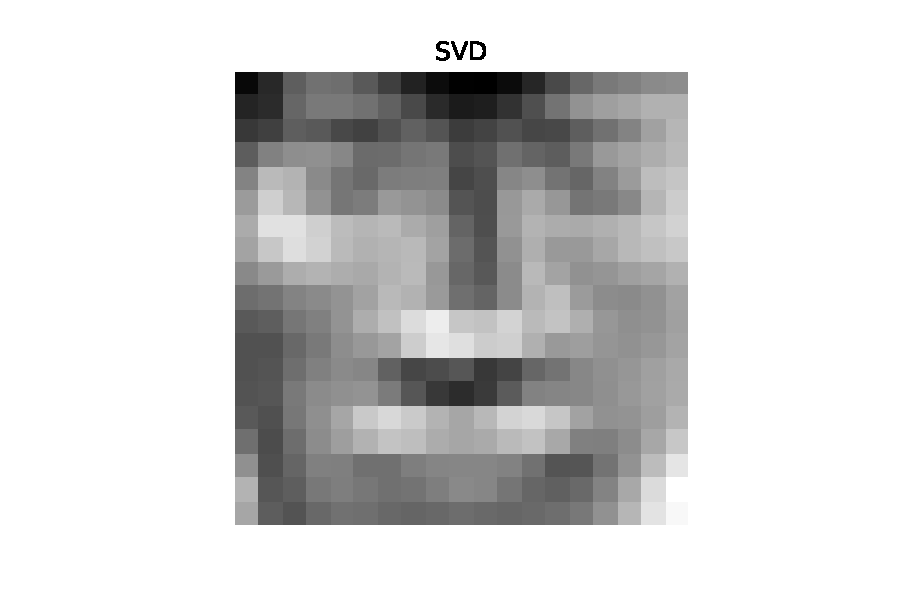
\includegraphics[width=0.45\textwidth]{Ex_03/Figures/svd.pdf}
\end{center}
%%%%%
%%%%%
%%%%%
%%%%%
%%%%%
\end{enumerate}

